\documentclass{article}
     \usepackage[final]{nips_2018}
\usepackage[dvipsnames]{xcolor}
\usepackage{array}
\usepackage{tabularx}% added for table design
\usepackage{lipsum}% for dummy text

\usepackage{graphicx}
\usepackage{caption}
\usepackage{subcaption}
\usepackage{array}
\usepackage{makecell}
\usepackage{amsmath}
\usepackage{graphicx}
\usepackage{caption}
\usepackage{subcaption}
\setlength{\belowcaptionskip}{0.0pt}

\usepackage[utf8]{inputenc} % allow utf-8 input
\usepackage[T1]{fontenc}    % use 8-bit T1 fonts
\usepackage{hyperref}       % hyperlinks
\usepackage{url}            % simple URL typesetting
\usepackage{booktabs}       % professional-quality tables
\usepackage{amsfonts}       % blackboard math symbols
\usepackage{nicefrac}       % compact symbols for 1/2, etc.
\usepackage{microtype}      % microtypography
\usepackage{xcolor}
\usepackage{hyperref}
\title{Different classifiers performance on two datasets}
\usepackage{placeins}
\usepackage{color, colortbl}
\definecolor{Gray}{rgb}{0.88,10,1}
\usepackage{pifont}
\newcommand{\cmark}{\ding{51}}%
\newcommand{\xmark}{\ding{55}}%

\author{%
  \textbf{Ahmed Amine Daou},  \texttt{\href{mailto:ahmed.aminedaou@umontreal.ca}{ahmed.amine.daou@umontreal.ca}} \\  
  \textbf{Alejandra Jimenez}, \texttt{\href{mailto:alejandra.jimenez.nieto@umontreal.ca}{alejandra.jimenez.nieto@umontreal.ca}} \\
  \textbf{Gabriel Lagubeau}, \texttt{\href{mailto:gabriel.lagubeau@umontreal.ca}{gabriel.lagubeau@umontreal.ca}} 
}
\begin{document}



\maketitle
\begin{abstract}
  In machine learning context theres is many algorithms to handle  classification problems, Algorithms accuracy depends mainly on dataset applied thereto. In this paper, We'll describe different classifiers' behaviour : Multilayer perceptron (MLP); Random
Forests (RF) and Naive Bayes. We choose two datasets: \href{https://www.cs.toronto.edu/~kriz/cifar.html}{CIFAR-10} and \href{https://archive.ics.uci.edu/ml/datasets/adult}{Adult Dataset}. for CIFAR-10 pre-processing phase, to improve accuracy
we applied Principal Component Analysis (PCA), and for Adult dataset we applied \textcolor{red}{alejandra apres}. After that, we evaluate and compare the performance of the models according to the specific metrics including accuracy, confusion matrix, cost-sensitive measure and computation runtime. As result we found that ... outperformed in CIFAR-10 with an accuracy blabla, and \textcolor{red}{algo x } gave the best result with \%
\end{abstract}

\section{Approach}
There is many approaches for images classification. The first step is the redefinition of the problem in a machine learning context, after that we'll be able to know what every chosen algorithm needs to run properly. The  next  step
is  to apply pre processing methods on our dataset,  doing so we'll extract a maximum of valuable information and make the classification accuracy evolve.
On a "well pre processed" dataset,  we can apply  a  plenty  of 
learning algorithms to extract a maximum of valuable information from our features which improve algorithms' accuracy during the testing phase.


 \subsection{Chosen Dataset description}
\begin{itemize}
\item \href{https://www.cs.toronto.edu/~kriz/cifar.html}{The CIFAR-10 dataset}
: A 10-class (airplane, automobile, bird, cat, deer, dog, frog, horse, ship, truck ) database of  60000 32x32 pixels images ,50000 for training divided and 10000 for testing selected randomly from each class.
\item \href{http://archive.ics.uci.edu/ml/datasets/Adult}{Adult Data Set} : Used to predict whether a person makes over 50K a year, relying on 48842 instances (32561 for training and 16281 for testing)  having 14 attributes .\end{itemize}



\section{Methods}
The main purpose is to implement and compare the performance of three classifiers. On each dataset, we applied Naive Bayes, and random forests, then a multilayer perceptron. After that, we performed hyper-parameters and PCA number of components tuning. The evaluation is based on precision, recall, f1-score values and confusion matrix.
\subsection{Naive Bayes:}
Naive Bayes methods are a set of supervised learning algorithms based on Bayes Theorem, known for being very naive and having a very low capacity because of supposing that features $X$ belonging to the same given class $c\in \{1,\hdots ,m\}$ are independent.


\subsection{Random Forests:}
Random  Forests (RF)  is  a model that fits decision trees on sampled dataset, $dimension_{sample}=dimension_{input}$. Trees are constructed with A recursive, top-down procedure that builds a tree before being pruned back to avoid overfitting.
its classification process, can be seen as a set of comparison (tests on features values) at every internal node.\\


\subsection{Multilayer perceptron:}
A multilayer perceptron is a one-way artificial neural network, it's a supervised machine learning algorithm, its modeling is based on human brain architecture.
Neurons are embedded into layers fully connected to each other. The first layer is composed of feature vector and called the input layer, The output layer is the component that gives the prediction, between them there's at least one hidden layer.
Hidden and output layers take $X$ as input and outputs $h_{W,b}$ where $W$ is the weights set and $b$ is the bias. 
$$h_{W,b}\left(X\right)=f\left(z\right)\; ; z=\sum_{i=1}^{n} W_ix_i+b$$
among many common activation function $f$ we'll use relu for hidden layers and softmax for output layer $$Relu\left(\mathbf{z}_j\right)=max\left(z_j,0\right)$$  
$$softmax\left(\mathbf{z}_j\right) = \frac{e^{z_j}}{\sum_{j=1}^k e^{z_k}}$$  $k$ here represents,the output layer dimension, or the number of possible classes.
\subsubsection*{Cross entropy loss:} Loss function used in ANN having $softmax$ as an activation function is cross Entropy loss, it indicates the difference between what the model believes and what real value is equal to.
$$L = - \sum_i y_i log(p_i) $$
If this loss function is non-convex it makes finding optimal values impossible sometimes, but it usually gives good results.

Weights which are initialized to low values are updated during backpropagation.\\
Hyper parameters are responsible of the algorithm behaviour.

\begin{itemize}
\item A high learning rate can make backpropagation algorithm jump around optimal values without getting them and  a one size makes backpropagation converges slowly.
\item A High iteration number can cause overfitting , and a low one causes underfitting.
\end{itemize}




\subsection{Preprocessing}



\FloatBarrier
\begin{table}[!htbp]
 \centering
  \caption{Preprocessing methods applied on each datasets}
  \label{sample-table}
  
  \begin{tabular}{lcl}
  
    \toprule
    \multicolumn{2}{c}{CIFAR-10}                   \\
    \cmidrule(r){1-2}
    Preprocessing method     & Description      \\
    \midrule
    \rowcolor{Gray}
    Features scaling &   \makecell{Each image is represented in a 3 dimensional  RGB vetor, each value is between 0 \& 255,\\ by deviding each value by 255 we'll get values between 0 \& 1. }   \\
    PCA    & \makecell{Principal components analysis is a famous method used to reduce dimentionality \\by projecting features in a n-dimentional space it's used in some cases for image denoising. }   \\
     \rowcolor{Gray}
    One-hot encoding      & \makecell{Training and testing labels are 1-dimensional vectors, $\left(50000,1\right)$ for training  \& $\left(10000,1\right)$ \\for testing. \textbf{MLP} output layer activation function is softmax, so to make the\\ cross entropy calculation possible,  each training label should be \\a $Classes_{number}$-dimentional vector, the result is a vector representing\\ having a unique $1$ in corresponding class index\\  }    \\
    
     \toprule
    \multicolumn{2}{c}{Adult dataset}                   \\
    \cmidrule(r){1-2}
    Preprocessing method     & Description      \\
    \midrule
    Dendrite & Input terminal      \\
    Axon     & Output terminal    \\
    Soma     & Cell body        \\
    \bottomrule
  \end{tabular}
\end{table}
\subsection{Design choices}
\begin{itemize}
\item The chosen language is Python, and the libraries used are:
\item Instead of downloading the Cifar data and load it from the disk, we imported it using keras function $cifar10.load\_data\left(\right)$
\item Classifiers are implemented in separate jupyter notebooks.
\end{itemize}

\section{Experiments, Results \& Comparision}


In the next table we'll show the pre processing impact on algorithms' accuracy and execution time, the table is displayed for illustrative purpose and the values  here are not the optimal obtained values.
it does not take account of PCA fitting execution time.




\begin{table}[ht]
  \caption{ Pre processing Method influence on each classifier}
  \label{sample-table}
  \centering
  \begin{tabular}{lccll}
    \toprule
    \multicolumn{5}{c}{CIFAR-10}                   \\
    \cmidrule(r){1-5}
    Classifier details     & Features Scaling   &  PCA & Execution time & Accuracy \\
    \midrule
    Multilayer Perceptron &   \xmark  & \xmark & $543.3s$ & $10\%$  \\
    
 PCA components=100   & \checkmark & \xmark  &$581.8s\left(\textcolor{red}{+38s}\right)$ & $39.04\% \left(\textcolor{ForestGreen}{+29.04\%}\right)$ \\  
      & \xmark & \checkmark & $168.7s\left(\textcolor{ForestGreen}{-413,1s}\right)$ & $25.69\% \left(\textcolor{red}{-13.35\%}\right)$ \\  
     & \checkmark & \checkmark & $146.6s \left(\textcolor{ForestGreen}{-22.1s}\right)$  & $57.63\% \left(\textcolor{ForestGreen}{+31.94\%}\right)$ \\      
      
      \toprule
  
   Naive Bayes(Gaussian) &   \xmark  & \xmark &  7.9s &  31\%  \\
 PCA components=40   & \checkmark & \xmark  & $6.8s\left(\textcolor{ForestGreen}{-1.1s}\right)$& 31\% \\  
      & \xmark & \checkmark &$0.1s\left(\textcolor{ForestGreen}{-6.7s}\right)$ & $36\% \left(\textcolor{ForestGreen}{+5\%}\right)$\\  
     & \checkmark & \checkmark &0.1s  &36 \% \\ 
 %$ 25.69\% \left( −13.35s \right)$ 
     \toprule
  
   Random Forests &   \xmark  & \xmark & $75.0s$ & $40.11\%$ \\
$n\_estimators=20$    & \checkmark & \xmark  & $72.0s\left(\textcolor{ForestGreen}{-3s}\right)$ &  $39.9\% \left(\textcolor{red}{-0.21\%}\right)$\\  
PCA components=40      & \xmark & \checkmark & $22.9s \left(\textcolor{ForestGreen}{-49.1s}\right)$ & $36.89\% \left(\textcolor{red}{-3.01\%}\right)$ \\  
     & \checkmark & \checkmark & $20.4s\left(\textcolor{ForestGreen}{-2.5s}\right)$ & $37.6\% \left(\textcolor{ForestGreen}{+0.71\%}\right)$\\ 
    \bottomrule
    \multicolumn{5}{c}{Adult Database}                   \\
    \cmidrule(r){1-5}
    Classifier     & Mthod1   &  Method2 & Execution Time & Accuracy \\
    \midrule
    Multilayer Perceptron &   \xmark  & \xmark & &  \\
    & \checkmark & \xmark  & &  \\  
      & \xmark & \checkmark & &  \\  
     & \checkmark & \checkmark & & \\      
      
      \toprule
  
   Naive Bayes &   \xmark  & \xmark & &  \\
    & \checkmark & \xmark  & &  \\  
      & \xmark & \checkmark & &  \\  
     & \checkmark & \checkmark & & \\ 
 
     \toprule
  
   Random Forests &   \xmark  & \xmark & &  \\
    & \checkmark & \xmark  & &  \\  
      & \xmark & \checkmark & &  \\  
     & \checkmark & \checkmark & & \\ 
    \bottomrule
  \end{tabular}
\end{table}
\FloatBarrier
\subsection{On CIFAR-10}
\subsubsection*{Hyper parameter tuning:}


In the next part we'll show the best results obtained for each classifier after model optimization using grid search.\textcolor{red}{(pas oublier) trouver des reponses à quelques questions}
\subsubsection{Multilayer Perceptron}
He we tuned learining rate  $\eta \in \{1,0.1,0.01,0.001\}$ \& epochs number in
$nb_{iteration} \in \{100,200,300,400\}$\textcolor{red}{<-a determiner}
\subsubsection{Naive Bayes}
Here we have no hyperparameter to tune so we tried different distribution (Gaussian, Multinomial \& Bernoulli ).
\begin{itemize}
\item \textbf{Gaussian Distribution: }


\begin{figure}[ht]
    \centering
    \begin{subfigure}{.6\columnwidth}
        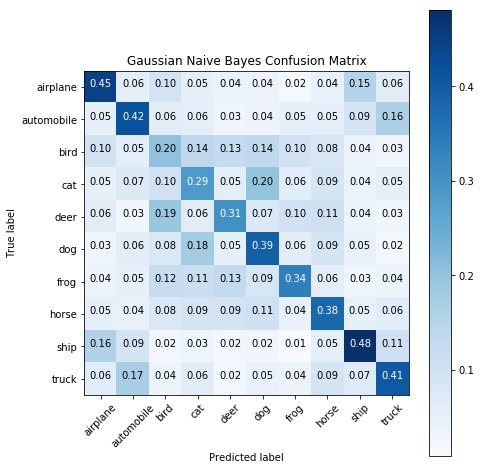
\includegraphics[width=\linewidth]{index}
  
    \end{subfigure}

    \bigskip% <-- added
    \begin{subfigure}{\columnwidth}
        \centering
        \renewcommand\tabularxcolumn[1]{m{#1}}% <-- added
        \renewcommand\arraystretch{1}
        \setlength\tabcolsep{2pt}% <-- added
        \begin{tabularx}{\linewidth}{*{6}{>{\centering\arraybackslash}X}}\hline
     &  & precision &   recall & f1-score  & support \\ \hline
                  
  \multicolumn{2}{c}{avg / total}& 0.37  &     0.37   &  0.36   &   10000 \\
  \end{tabularx}
     
        \caption{Gaussian Naive Bayes classification report  }
    \end{subfigure}

    \label{my label}
\end{figure}
\FloatBarrier

\item \textbf{Multinomial Distribution: }


\begin{figure}[ht]
    \centering
    \begin{subfigure}{.6\columnwidth}
        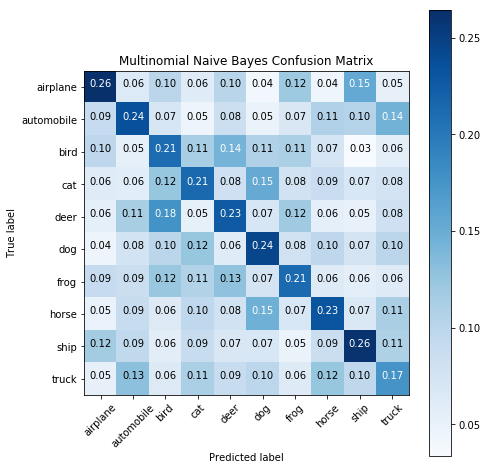
\includegraphics[width=\linewidth]{multi}
  
    \end{subfigure}

    \bigskip% <-- added
    \begin{subfigure}{\columnwidth}
        \centering
        \renewcommand\tabularxcolumn[1]{m{#1}}% <-- added
        \renewcommand\arraystretch{1}
        \setlength\tabcolsep{2pt}% <-- added
        \begin{tabularx}{\linewidth}{*{6}{>{\centering\arraybackslash}X}}\hline
     &  & precision &   recall & f1-score  & support \\ \hline
                  
  \multicolumn{2}{c}{avg / total}& 0.30   &   0.30    &  0.30   &  10000
  \end{tabularx}
     
        \caption{Multinomial Naive Bayes classification report  }
    \end{subfigure}

    \label{my label}
\end{figure}
\FloatBarrier



\item \textbf{Bernoulli Distribution: }
\begin{figure}[ht]
    \centering
    \begin{subfigure}{.6\columnwidth}
        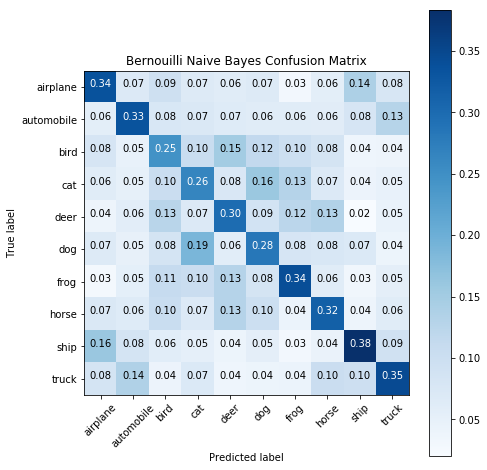
\includegraphics[width=\linewidth]{Bernoui}
  
    \end{subfigure}

    \bigskip% <-- added
    \begin{subfigure}{\columnwidth}
        \centering
        \renewcommand\tabularxcolumn[1]{m{#1}}% <-- added
        \renewcommand\arraystretch{1}
        \setlength\tabcolsep{1pt}% <-- added
        \begin{tabularx}{\linewidth}{*{6}{>{\centering\arraybackslash}X}}\hline
     &  & precision &   recall & f1-score  & support \\ \hline
                  
  \multicolumn{2}{c}{avg / total}& 0.30    &  0.30  &    0.30  &   10000
  \end{tabularx}
     
        \caption{Bernoulli Naive Bayes classification report  }
    \end{subfigure}

    \label{my label}
\end{figure}
\FloatBarrier


\end{itemize}


\subsubsection{Random Forests}
RF we tuned nEstimators with these values $\{25,50,100,150,200,250\}$ and pca components in $\{\hdots\}$
\begin{figure}[ht]
    \centering
        \centering
        \renewcommand\tabularxcolumn[1]{m{#1}}% <-- added
        \renewcommand\arraystretch{1}
        \setlength\tabcolsep{2pt}% <-- added
        \begin{tabularx}{\linewidth}{*{6}{>{\centering\arraybackslash}X}}\hline
   \makecell{PCA Components or other}   & n estimators & Accuracy &   execution time  \\ \hline
                  
 valu11  & value21& 0.30   &   0.30   \\ 
  valu12  & value22& 0.3560   &   0.8630   \\ 

  \end{tabularx}
     
        \caption{Multinomial Naive Bayes classification report  }
\end{figure}
\FloatBarrier

\subsection{On Adult dataset}
\subsection{multilayer perceptron}
\textcolor{red}{alejandra}
\subsubsection{Naive Bayes}
\textcolor{red}{alejandra}
\subsubsection{Random forests}
\textcolor{red}{alejandra}





\section{Design Choices}



\subsection*{Acknowledgments}



\section*{References}

References follow the acknowledgments. Use unnumbered first-level heading for
the references. Any choice of citation style is acceptable as long as you are
consistent. It is permissible to reduce the font size to \verb+small+ (9 point)
when listing the references. {\bf Remember that you can use more than eight
  pages as long as the additional pages contain \emph{only} cited references.}
\medskip

\small

[1] Alexander, J.A.\ \& Mozer, M.C.\ (1995) Template-based algorithms for
connectionist rule extraction. In G.\ Tesauro, D.S.\ Touretzky and T.K.\ Leen
(eds.), {\it Advances in Neural Information Processing Systems 7},
pp.\ 609--616. Cambridge, MA: MIT Press.

[2] Bower, J.M.\ \& Beeman, D.\ (1995) {\it The Book of GENESIS: Exploring
  Realistic Neural Models with the GEneral NEural SImulation System.}  New York:
TELOS/Springer--Verlag.

[3] Hasselmo, M.E., Schnell, E.\ \& Barkai, E.\ (1995) Dynamics of learning and
recall at excitatory recurrent synapses and cholinergic modulation in rat
hippocampal region CA3. {\it Journal of Neuroscience} {\bf 15}(7):5249-5262.
http://www.visiondummy.com/2014/05/feature-extraction-using-pca/
https://www.techopedia.com/definition/32509/principal-component-analysis-pca
\end{document}
